 \section{Jamming Basics}

\paragraph{Jamming}
Entirely \hl{preventing or reducing the ability of communicating parties to pass information}, either intentionally or unintentionally.

The jamming signal needs to have the same frequency as the modulated signal.
If the latter is unknown to the attacker, they thus need to jam a wide bandwidth of frequencies (containing the band used by the legitimate parties) to be successful.

Effectively, jamming is always a power play.

\paragraph{Symbol}
Carries one or more bit of information, depending on the modulation scheme.

\paragraph{Symbol Jamming}
Corrupts symbols such that the receiver can EITHER not interpret them at all OR interprets them incorrectly.\\
Targeted, low-power jamming of specific symbols is hard!

\paragraph{Communication Jamming}
Corrupts enough bits that the information cannot be reconstructed any more, despite error correction.

\paragraph{Jamming-to-Signal Ratio J/S} = $J -  S$, i.e.\ the difference between the jamming signal and the modulated signal in dB.
Usually, a ratio $J/S = 0$ results in successful jamming.

\paragraph{Burn-through range}
Range in which communication still succeeds, despite jamming.

\paragraph{Attacker model}
% taken from the following chapter/deck of slides
Types: responsive, sweep, random 

Actions: jam, insert, modify (= overshadow) 

Power to jam/insert/modify: $P_j, P_t, P_o$ 

Number of channels to jam/insert/modify: $c_j, c_t, c_o$ 

Total strength/power $P_T$ 

\[ c_j P_j + c_t P_t + c_o P_o \leq P_T\]

\subsection{Communication Jamming --- LTE}
Knowledge about the protocol can allow for more efficient jamming. In LTE, connection establishment relies on information that is transmitted on control channels. Targeting these channels with a (protocol-aware) jamming attack, can allow a DoS without wasting a lot of power using the \emph{Capture Effect}.
\subsection{Jamming Resistant Communication}\label{sec:jamming-resistant-comm}

\paragraph{Basic principle}
If you cannot fight (i.e.\ have too little power), RUN, HIDE or WAIT, and get ad advantage over the attacker: use a shared secret.

\paragraph{Frequency Hopping Spread Spectrum FHSS}
Regularly change transmission frequency.
The pseudorandom frequency sequence is derived from a shared secret.
Sender and receiver \textbf{must} be synchronized.

Note that frequency hoppers can be detected and located, simply by looking over time from which direction someone is sending on changing frequencies.

Possible attacks:
\begin{itemize}
	\item \textbf{Partial band jammer:}
	Distribute jamming power over a subset of all hopping frequencies to achieve $J/S=0$ at least on that range.
	\item \textbf{Follower jammer:}
	Detects on which frequency communication occurs and then jams it.
	Can be protected against by using error codes (since only the final bits will be corrupted).
\end{itemize}

\subsection{Direct Sequence Spread Spectrum DSSS}
This technique allows  \textbf{spreading the baseband over a larger bandwidth using a shared secret} (narrow-band to broadband). \\
Since the \hl{transmission power remains the same}, the \hl{power density at any given frequency decreases}.
Thus, the spread signal can effectively \emph{hide under the noise} (\autoref{fig:dsss-psd}).

To spread over more frequencies, we need a higher symbol/bit rate. To achieve this, the information signal is multiplied with high-frequency pseudorandom sequences called \textbf{chips} or \textbf{spreading codes}.
The result resembles \textbf{white noise}.
See \autoref{fig:dsss}.

During de-spreading, the signal is again multiplied with the same spreading code.
De-spreading converts the wide-band signal into a narrow-band one (this works due to the autocorrelation properties of the spreading code).
At the same time, any narrow-band interference is spread out.
\\
Thus, DSSS is more robust against [un]intentional interference and multi-path effects. Broadband jamming is possible, but inherently requires much power.

Detecting DSSS signals is difficult, but not impossible (energy detection of strong signals, signal characteristics such as constant chip rate). Thus, interception and modification is hard.

Example usages: GPS, 802.11b WiFi, CDMA (used in 3G).
Non-military applications mainly use DSSS for interference-resistance and use public spreading codes.
They are thus still vulnerable to malicious jamming, to cause a DoS.

\begin{figure}[h]
	\centering
	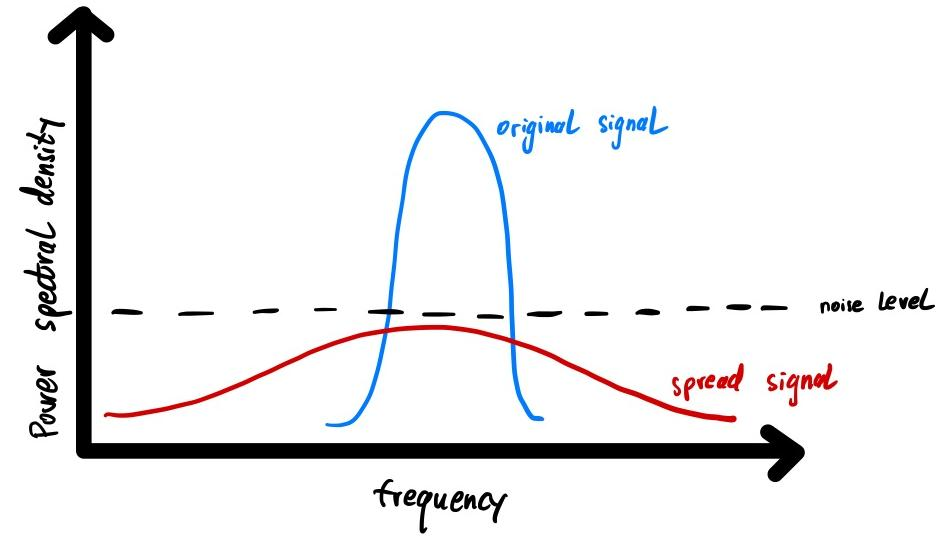
\includegraphics[scale=0.4]{images/2-dsss-psd.jpg}
	\caption{DSSS --- hiding under the noise}%
	\label{fig:dsss-psd}
\end{figure}

\begin{figure}[h]
	\centering
	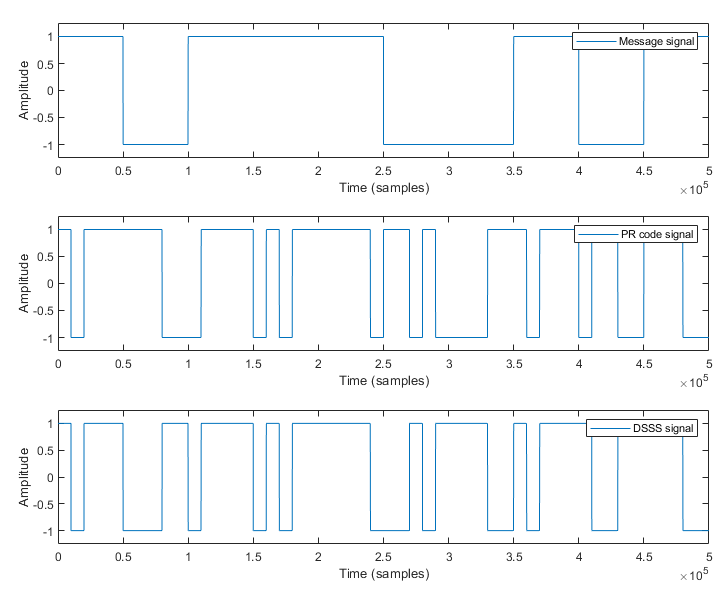
\includegraphics[scale=0.6]{images/2-dsss.png}
	\caption{DSSS --- baseband signal, spreading code, spread signal (top to bottom)}%
	\label{fig:dsss}
\end{figure}

\paragraph{Processing Gain PG}
Ratio of the spread bandwidth to the narrow bandwidth, in dB, or \hl{chip-rate over bit rate}.


\paragraph{Chirp Signal / Sweep Signal}
Signal in which the frequency increases and decreases over time (``sweeping'' over a bandwidth much wider than the baseband bandwidth).
Narrow-band and partial-band jamming are prevented, follower jamming not so much

\paragraph{Code-Division Multiple Access CDMA}
Multiple transmitters sending in the same area simultaneously, but using different spreading codes.
Allows sharing of the same frequencies/bandwidth without interference.
